\documentclass[12pt,a4paper]{article}

% --- Idioma y codificacion ---
\usepackage[spanish]{babel}
\usepackage[utf8]{inputenc}
\usepackage[T1]{fontenc}

% --- Maquetacion ---
\usepackage[a4paper,top=2.5cm,bottom=2.5cm,left=2.2cm,right=2.2cm,columnsep=0.7cm]{geometry}
\usepackage{setspace}
\usepackage{titlesec}
\usepackage[hidelinks]{hyperref}
\usepackage{fancyhdr}
\usepackage{multicol}
\usepackage{multirow}
\usepackage{rotating}

% --- Ciencia y tablas ---
\usepackage{amsmath,amssymb}
\usepackage{siunitx}
\usepackage{booktabs}
\usepackage{array}
\usepackage{tabularx}
\usepackage{graphicx}
\usepackage{float}

\sisetup{output-decimal-marker={,}}
\setstretch{1.15}
\setlength{\parindent}{0pt}
\setlength{\parskip}{6pt}
\renewcommand{\arraystretch}{1.25}
\setlength{\abovedisplayskip}{5pt}
\setlength{\belowdisplayskip}{5pt}
\setlength{\abovedisplayshortskip}{3pt}
\setlength{\belowdisplayshortskip}{3pt}
\setlength{\emergencystretch}{3em}

\titleformat{\section}{\normalfont\large\bfseries}{\thesection}{1em}{}
\titleformat{\subsection}{\normalfont\normalsize\bfseries}{\thesubsection}{1em}{}
\titlespacing*{\section}{0pt}{6pt}{2pt}
\titlespacing*{\subsection}{0pt}{4pt}{1pt}

\setlength{\abovecaptionskip}{2pt}
\setlength{\belowcaptionskip}{6pt}

\addto\captionsspanish{\renewcommand{\contentsname}{Índice}}
\addto\captionsspanish{\renewcommand{\tablename}{Tabla}}
\hypersetup{hypertexnames=false}

\pagestyle{fancy}
\fancyhf{}
\lhead{Práctica 2: Osciloscopio y Figuras de Lissajous}
\rhead{Electromagnetismo II}
\cfoot{\thepage}
\setlength{\headheight}{14.5pt}

\newcolumntype{Y}{>{\centering\arraybackslash}X}
\newcolumntype{C}[1]{>{\centering\arraybackslash}p{#1}}
\newcolumntype{M}[1]{>{\centering\arraybackslash}m{#1}}

\begin{document}

% ============================================================
\begin{titlepage}
    \centering
    \vspace*{3cm}
    {\LARGE\bfseries Figuras de Lissajous\par}
    \vspace{0.5cm}
    {\large Práctica 2: Manejo del osciloscopio\par}
    \vspace{1.2cm}
    {\large Asignatura: Electromagnetismo II\par}
    \vspace{0.4cm}
    {\large Autor: Luis López Nasser\par}
    \vspace{0.2cm}
    {\large Fecha: 21/04/2026\par}
    \vspace{0.2cm}
    {\large Universidad UNIE\par}
    \vfill
\end{titlepage}

\tableofcontents
\clearpage

% ============================================================
\begin{multicols}{2}

\section{Introducción}

\subsection{Marco teórico}

El osciloscopio digital permite visualizar señales eléctricas de diferencia de potencial en función del tiempo, incorporando un conversor analógico-digital que transforma la señal en datos procesables. En modo X--T representa amplitud frente a tiempo; en modo X--Y desactiva la base de tiempos y muestra una señal frente a otra, lo que permite analizar directamente relaciones de fase y frecuencia entre dos canales.

Para una señal sinusoidal, la lectura por rejilla proporciona el voltaje pico a pico y el periodo mediante:
\begin{equation}
V_{pp} = n_V \cdot (\text{V/div}), \qquad T = n_T \cdot (\text{s/div}),
\label{eq:rejilla}
\end{equation}
donde $n_V$ y $n_T$ son las divisiones verticales y horizontales leídas en pantalla. Los parámetros derivados son:
\begin{equation}
f = \frac{1}{T}, \qquad V_p = \frac{V_{pp}}{2}, \qquad V_{ef} = \frac{V_{pp}}{2\sqrt{2}}.
\label{eq:derivadas}
\end{equation}

Las medidas directas se tratan con incertidumbre tipo B:
\begin{equation}
\delta x = \frac{\text{resolución}}{2}.
\label{eq:tipoB}
\end{equation}
La propagación de incertidumbre para las magnitudes derivadas es:
\begin{equation}
\delta f = \frac{\delta T}{T^{2}}, \quad \delta V_p = \frac{\delta V_{pp}}{2}, \quad \delta V_{ef} = \frac{\delta V_{pp}}{2\sqrt{2}}.
\label{eq:propagacion}
\end{equation}

Para contrastar cuantitativamente dos valores medidos $x_i$ y $x_j$ se usa el estadístico de compatibilidad:
\begin{equation}
C_{ij} = \frac{|x_i - x_j|}{\sqrt{(\delta x_i)^2 + (\delta x_j)^2}}.
\label{eq:compat}
\end{equation}
Se considera compatibilidad experimental razonable cuando $C_{ij} \leq 1$.

En modo X--Y se superponen dos oscilaciones ortogonales:
\begin{equation}
X(t) = A\sin(\omega_1 t), \quad Y(t) = B\sin(\omega_2 t + \phi),
\label{eq:lissajous}
\end{equation}
donde $\phi$ es el desfase relativo. La curva de Lissajous se cierra cuando $\nu_1/\nu_2$ es racional; su forma depende además del valor de $\phi$. Dado que $\phi$ no se controla directamente al usar generadores independientes, la figura evoluciona lentamente en el tiempo recorriendo todas las configuraciones asociadas a los posibles valores del desfase.

\subsection{Objetivos}

\begin{itemize}
    \item Familiarizarse con el manejo básico del osciloscopio.
    \item Medir $T$, $f$, $V_{pp}$, $V_p$ y $V_{ef}$ con tres métodos y comparar su precisión mediante análisis de incertidumbres.
    \item Visualizar figuras de Lissajous para relaciones de frecuencia $1{:}1$, $1{:}2$, $1{:}3$ y $2{:}3$.
    \item Determinar las condiciones que deben satisfacer las amplitudes y el desfase para obtener una circunferencia.
\end{itemize}

\section{Material}

\begin{itemize}
    \item Osciloscopio digital de dos canales.
    \item Dos generadores de señales sinusoidales.
    \item Cables coaxiales de conexión.
\end{itemize}

Las incertidumbres tipo B asociadas a cada instrumento se recogen en la Tabla~\ref{tab:incertidumbres}.

\begin{table}[H]
\centering
\caption{Resolución e incertidumbre tipo B de cada instrumento.}
\label{tab:incertidumbres}
\small
\begin{tabularx}{\columnwidth}{>{\raggedright\arraybackslash}p{0.43\columnwidth}YY}
\toprule
Magnitud & Resolución & $\delta x$ \\
\midrule
$f_{nom}$ del generador & \SI{1}{Hz} & \SI{0,5}{Hz} \\
$T_{rej}$ por rejilla & \SI{1}{\micro\second} & \SI{0,5}{\micro\second} \\
$V_{pp}$ por rejilla & \SI{0,001}{V} & \SI{0,0005}{V} \\
$f_{cur}$ por cursores & \SI{0,1}{Hz} & \SI{0,05}{Hz} \\
$f_{auto}$ automática & \SI{0,001}{Hz} & \SI{0,0005}{Hz} \\
\bottomrule
\end{tabularx}
\end{table}

\section{Procedimiento experimental}

Con amplitud fija en el generador se barrieron las frecuencias nominales \SIlist{50;100;200;800;3000}{\hertz}. Para cada ajuste se visualizó la señal en modo X--T, ajustando las escalas Volts/Div y Time/Div para ocupar la mayor parte de la pantalla sin saturación de picos. Se centró la traza y se estabilizó mediante el trigger.

\textbf{Método A --- Rejilla:} Se contaron las divisiones horizontales entre crestas consecutivas para obtener $T_{rej}$, y las divisiones verticales totales para $V_{pp}$, multiplicando en cada caso por la escala activa.

\textbf{Método B --- Cursores:} En modo CURSORES, tipo X/Tiempo, los cursores se situaron en dos crestas consecutivas para leer $\Delta t = T$; el equipo muestra automáticamente la inversa $1/\Delta t$ como frecuencia.

\textbf{Método C --- Medida automática:} Pulsando MEASURE, seleccionando CH1 y activando los parámetros Frecuencia y $V_{pp}$, los valores aparecen directamente en pantalla.

En la segunda parte se conectó cada generador a un canal del osciloscopio, se activó el modo X--Y (menú Horizontal $\to$ Time Base $\to$ X-Y) y se buscaron figuras de Lissajous para relaciones de frecuencia $1{:}1$, $1{:}2$, $1{:}3$ y $2{:}3$, generando al menos ocho figuras en total.

\end{multicols}

% ============================================================
\section{Resultados experimentales}
% ============================================================

\begin{table}[H]
\centering
\small
\setlength{\tabcolsep}{3.5pt}
\caption{Medidas de periodo y frecuencia por los tres métodos. La incertidumbre de $f_{rej}$ se obtiene por propagación según~\eqref{eq:propagacion}.}
\label{tab:tiempos}
\begin{tabular}{C{1.3cm}C{3.2cm}C{3.0cm}C{3.0cm}C{3.2cm}}
\toprule
$f_{nom}$ (Hz) & $(T \pm \delta T)_{rej}$ (ms) & $(f \pm \delta f)_{rej}$ (Hz) & $(f \pm \delta f)_{cur}$ (Hz) & $(f \pm \delta f)_{auto}$ (Hz) \\
\midrule
50   & $20{,}000 \pm 0{,}010$  & $50{,}00 \pm 0{,}013$   & $50{,}00 \pm 0{,}05$   & $49{,}9686 \pm 0{,}0001$ \\
100  & $10{,}000 \pm 0{,}010$  & $100{,}00 \pm 0{,}050$  & $100{,}0 \pm 0{,}05$   & $100{,}024 \pm 0{,}001$  \\
200  & $4{,}9930 \pm 0{,}0005$ & $200{,}28 \pm 0{,}020$  & $200{,}3 \pm 0{,}05$   & $200{,}009 \pm 0{,}001$  \\
800  & $1{,}2500 \pm 0{,}0005$ & $800{,}00 \pm 0{,}320$  & $800{,}0 \pm 0{,}05$   & $800{,}028 \pm 0{,}001$  \\
3000 & $0{,}3330 \pm 0{,}0005$ & $3000{,}14 \pm 0{,}045$ & $3000{,}14 \pm 0{,}01$ & $3000{,}14 \pm 0{,}01$   \\
\bottomrule
\end{tabular}
\end{table}

\begin{table}[H]
\centering
\small
\setlength{\tabcolsep}{5pt}
\caption{Voltaje pico a pico, de pico y eficaz con incertidumbres propagadas según~\eqref{eq:propagacion}.}
\label{tab:voltajes}
\begin{tabular}{C{1.3cm}C{3.0cm}C{3.0cm}C{3.0cm}}
\toprule
$f_{nom}$ (Hz) & $(V_{pp} \pm \delta V_{pp})$ (V) & $(V_p \pm \delta V_p)$ (V) & $(V_{ef} \pm \delta V_{ef})$ (V) \\
\midrule
50   & $6{,}160 \pm 0{,}005$ & $3{,}080 \pm 0{,}0025$ & $2{,}178 \pm 0{,}0018$ \\
100  & $6{,}080 \pm 0{,}005$ & $3{,}040 \pm 0{,}0025$ & $2{,}150 \pm 0{,}0018$ \\
200  & $6{,}080 \pm 0{,}005$ & $3{,}040 \pm 0{,}0025$ & $2{,}150 \pm 0{,}0018$ \\
800  & $6{,}000 \pm 0{,}005$ & $3{,}000 \pm 0{,}0025$ & $2{,}121 \pm 0{,}0018$ \\
3000 & $6{,}080 \pm 0{,}005$ & $3{,}040 \pm 0{,}0025$ & $2{,}150 \pm 0{,}0018$ \\
\bottomrule
\end{tabular}
\end{table}

\begin{table}[H]
\centering
\small
\setlength{\tabcolsep}{5pt}
\caption{Comparación de frecuencias: estadístico $C_{ij}$ según~\eqref{eq:compat}. Compatibilidad si $C_{ij} \leq 1$.}
\label{tab:compat}
\begin{tabular}{C{1.3cm}C{2.5cm}C{2.5cm}C{2.5cm}C{2.5cm}}
\toprule
$f_{nom}$ (Hz) & $C(\text{rej}, nom)$ & $C(\text{cur}, nom)$ & $C(\text{auto}, nom)$ & $C(\text{auto}, \text{rej})$ \\
\midrule
50   & 0,00 & 0,00 & 0,063 & 2,42 \\
100  & 0,00 & 0,00 & 0,048 & 0,48 \\
200  & 0,56 & 0,60 & 0,018 & 13,5 \\
800  & 0,00 & 0,00 & 0,056 & 0,088 \\
3000 & 0,28 & 0,27 & 0,28  & 0,00 \\
\bottomrule
\end{tabular}
\end{table}

\begin{table}[H]
\centering
\small
\setlength{\tabcolsep}{5pt}
\caption{Variación de la amplitud al modificar la frecuencia nominal.}
\label{tab:amplitud}
\begin{tabular}{C{1.8cm}C{2.5cm}C{6.5cm}}
\toprule
$f_{nom}$ (Hz) & $V_{pp}$ (V) & Observación \\
\midrule
50   & 6,160 & Referencia \\
100  & 6,080 & $-0{,}08$ V ($-1{,}3\,$\%) — dentro del error de rejilla \\
200  & 6,080 & $-0{,}08$ V ($-1{,}3\,$\%) — dentro del error de rejilla \\
800  & 6,000 & $-0{,}16$ V ($-2{,}6\,$\%) — ligera disminución \\
3000 & 6,080 & $-0{,}08$ V ($-1{,}3\,$\%) — dentro del error de rejilla \\
\bottomrule
\end{tabular}
\end{table}

\begin{table}[H]
\centering
\small
\setlength{\tabcolsep}{4pt}
\caption{Registro de figuras de Lissajous. Se obtuvieron dos figuras por relación variando el desfase relativo.}
\label{tab:lissajous}
\begin{tabular}{C{0.8cm}C{1.4cm}C{1.9cm}C{1.9cm}C{4.5cm}}
\toprule
Fig. & Relación & $f_X$ (Hz) & $f_Y$ (Hz) & Forma observada \\
\midrule
1 & $1{:}1$ & 99,60  & 100,0 & Elipse inclinada ($\phi \approx \pi/4$) \\
2 & $1{:}1$ & 100,0  & 100,0 & Circunferencia/elipse ($\phi \approx \pi/2$) \\
3 & $1{:}2$ & 100,0  & 200,0 & Ocho horizontal \\
4 & $1{:}2$ & 100,0  & 200,0 & Lazo simple \\
5 & $1{:}3$ & 100,0  & 300,3 & Triple lazo simétrico \\
6 & $1{:}3$ & 100,0  & 300,3 & Arco triple ondulado \\
7 & $2{:}3$ & 200,0  & 300,3 & Figura trenzada (4 lóbulos) \\
8 & $2{:}3$ & 200,0  & 300,3 & Lazo asimétrico \\
\bottomrule
\end{tabular}
\end{table}

% ============================================================
\begin{multicols}{2}

\section{Análisis y discusión}

\subsection{Comparación de los tres métodos de frecuencia}

Los estadísticos de la Tabla~\ref{tab:compat} muestran que los métodos de rejilla y cursores son compatibles con el valor nominal del generador en todas las frecuencias ($C \leq 1$). La medida automática también lo es frente a $f_{nom}$, ya que las diferencias absolutas ($\lesssim 0{,}03$ Hz a baja frecuencia, $\lesssim 0{,}14$ Hz a \SI{3000}{Hz}) son pequeñas en comparación con $\delta f_{nom} = \SI{0,5}{Hz}$.

Sin embargo, al comparar directamente la medida automática con la de rejilla ($C_{\text{auto},\text{rej}}$), se obtienen valores superiores a la unidad en \SI{50}{Hz} ($C = 2{,}42$) y en \SI{200}{Hz} ($C = 13{,}5$). Esto indica que la incertidumbre declarada de la medida automática ---igual a la última cifra significativa mostrada en pantalla--- es demasiado optimista: las discrepancias reales entre métodos superan el límite de compatibilidad que dicha incertidumbre implicaría. Una estimación más conservadora de $\delta f_{auto} \approx \SI{0,05}{Hz}$, comparable a la del método de cursores, resulta más coherente con el conjunto de resultados.

El valor extremo $C = 13{,}5$ en \SI{200}{Hz} refleja que la lectura de rejilla ($f_{rej} = \SI{200,28}{Hz}$) acumula mayor error de apreciación visual que la medida automática ($f_{auto} = \SI{200,009}{Hz}$, muy próxima a la nominal). Esto ilustra la limitación inherente del método A: su incertidumbre depende fuertemente de la escala utilizada y de la habilidad del observador.

\subsection{Variación de amplitud con la frecuencia}

La tensión $V_{pp}$ se mantiene prácticamente constante en el rango \SIrange{50}{3000}{\hertz} (Tabla~\ref{tab:amplitud}), con variaciones inferiores al $3\,$\% que están dentro del error de apreciación de la rejilla. No se aprecia ninguna tendencia de atenuación sistemática con la frecuencia, lo que confirma que el canal del osciloscopio no introduce filtrado apreciable en este rango de trabajo.

\subsection{Figuras de Lissajous}

Las ocho figuras de la Tabla~\ref{tab:lissajous} corresponden correctamente a las relaciones ajustadas. Para cada relación se obtuvieron dos formas distintas variando el desfase relativo, en acuerdo con las formas teóricas esperadas para cada razón de frecuencias.

Para la relación $1{:}1$, con frecuencias iguales e idéntica amplitud ajustada por escala, se observó la transición elipse--circunferencia al imponer $\phi \approx \pi/2$. La lenta rotación de la figura evidencia que el desfase relativo entre generadores independientes varía con el tiempo, tal como predice la teoría.

Para $1{:}2$ y $1{:}3$ se identificaron los bucles y multilazos característicos. La relación $2{:}3$ fue la más exigente de estabilizar, requiriendo un ajuste muy fino de las frecuencias de ambos generadores.

\end{multicols}

\begin{multicols}{2}

\section{Conclusiones}

Los tres métodos de medida de frecuencia son compatibles con los valores nominales del generador dentro de sus incertidumbres. El método automático presenta la menor incertidumbre declarada, pero la comparación directa con el método de rejilla arroja estadísticos $C > 1$ en \SI{50}{Hz} y \SI{200}{Hz}, lo que demuestra que asignar como incertidumbre la última cifra significativa del display es excesivamente optimista. Una estimación más realista de $\delta f_{auto} \approx \SI{0,05}{Hz}$ restituye la compatibilidad entre métodos. El método de cursores ofrece una buena relación entre precisión y control directo del observador.

La amplitud $V_{pp}$ se mantiene constante dentro del error experimental ($< 3\,$\%) en todo el rango de frecuencias estudiado, sin evidencia de atenuación por filtrado del instrumento.

Las ocho figuras de Lissajous observadas corresponden correctamente a las relaciones $1{:}1$, $1{:}2$, $1{:}3$ y $2{:}3$. La evolución temporal de las figuras confirma que el desfase relativo entre generadores independientes no es estacionario. Para obtener una circunferencia en la relación $1{:}1$ deben cumplirse simultáneamente: igual frecuencia ($\nu_1 = \nu_2$), igual amplitud efectiva en pantalla ($A = B$ tras ajuste de escala) y desfase en cuadratura ($\phi = \pi/2 + k\pi$, $k \in \mathbb{Z}$).

\end{multicols}

% ============================================================
\appendix
% ============================================================

\section{Cuestionario --- Resultados experimentales}

\renewcommand{\arraystretch}{2.0}
\begin{table}[H]
\centering
\footnotesize
\setlength{\tabcolsep}{3pt}
\caption{Hoja de resultados experimentales en el formato del guion de la práctica.}
\label{tab:cuestionario}
\resizebox{\linewidth}{!}{%
\begin{tabular}{M{0.5cm}|>{\raggedright\arraybackslash}m{4.0cm}|M{3.0cm}|M{3.0cm}|M{3.0cm}|M{3.0cm}}
\toprule
& $\nu_{nom} \pm \Delta\nu_{nom}$ (Hz)
& $50 \pm 0{,}5$
& $100 \pm 0{,}5$
& $800 \pm 0{,}5$
& $3000 \pm 0{,}5$ \\
\midrule
\multirow{6}{*}{\rotatebox[origin=c]{90}{\normalsize\textbf{Tiempos}}}
& Escala de tiempo (s/div)
  & \SI{5}{ms}       & \SI{2}{ms}        & \SI{0,25}{ms}     & \SI{0,1}{ms} \\
& Divisiones de pantalla
  & 4,00             & 5,00              & 5,00              & 3,33 \\
& $(T \pm \Delta T\;\text{(s)})_{\text{rej}}$
  & $0{,}02000 \pm 1{\cdot}10^{-5}$
  & $0{,}01000 \pm 1{\cdot}10^{-5}$
  & $1{,}250{\cdot}10^{-3} \pm 1{\cdot}10^{-6}$
  & $3{,}33{\cdot}10^{-4} \pm 1{\cdot}10^{-6}$ \\
& $(\nu \pm \Delta\nu\;\text{(Hz)})_{\text{rej}}$
  & $50{,}00 \pm 0{,}013$
  & $100{,}00 \pm 0{,}05$
  & $800{,}00 \pm 0{,}32$
  & $3000{,}14 \pm 0{,}045$ \\
& $(\nu \pm \Delta\nu\;\text{(Hz)})_{\text{cur}}$
  & $50{,}00 \pm 0{,}05$
  & $100{,}0 \pm 0{,}05$
  & $800{,}0 \pm 0{,}05$
  & $3000{,}14 \pm 0{,}01$ \\
& $(\nu \pm \Delta\nu\;\text{(Hz)})_{\text{auto}}$
  & $49{,}969 \pm 0{,}001$
  & $100{,}024 \pm 0{,}001$
  & $800{,}028 \pm 0{,}001$
  & $3000{,}14 \pm 0{,}01$ \\
\midrule
\multirow{5}{*}{\rotatebox[origin=c]{90}{\normalsize\textbf{Voltajes}}}
& Escala de tensión (V/div)
  & \SI{2}{V}        & \SI{2}{V}         & \SI{2}{V}         & \SI{2}{V} \\
& Divisiones de pantalla
  & 3,08             & 3,04              & 3,00              & 3,04 \\
& $(V_{pp} \pm \Delta V_{pp}\;\text{(V)})_{\text{rej}}$
  & $6{,}160 \pm 0{,}005$
  & $6{,}080 \pm 0{,}005$
  & $6{,}000 \pm 0{,}005$
  & $6{,}080 \pm 0{,}005$ \\
& $V_p \pm \Delta V_p$ (V)
  & $3{,}080 \pm 0{,}0025$
  & $3{,}040 \pm 0{,}0025$
  & $3{,}000 \pm 0{,}0025$
  & $3{,}040 \pm 0{,}0025$ \\
& $V_{ef} \pm \Delta V_{ef}$ (V)
  & $2{,}178 \pm 0{,}0018$
  & $2{,}150 \pm 0{,}0018$
  & $2{,}121 \pm 0{,}0018$
  & $2{,}150 \pm 0{,}0018$ \\
\bottomrule
\end{tabular}%
}
\end{table}
\renewcommand{\arraystretch}{1.25}

\vspace{0.8cm}
\begin{table}[H]
\setlength{\abovecaptionskip}{4pt}
\setlength{\belowcaptionskip}{4pt}
\centering
\small
\renewcommand{\arraystretch}{1.6}
\setlength{\tabcolsep}{8pt}
\caption{Figuras de Lissajous: relación de frecuencias y valores de canal empleados.}
\label{tab:lissajous_cuestionario}
\begin{tabular}{lcccc}
\toprule
 & $1{:}1$ & $1{:}2$ & $1{:}3$ & $2{:}3$ \\
\midrule
Vista & 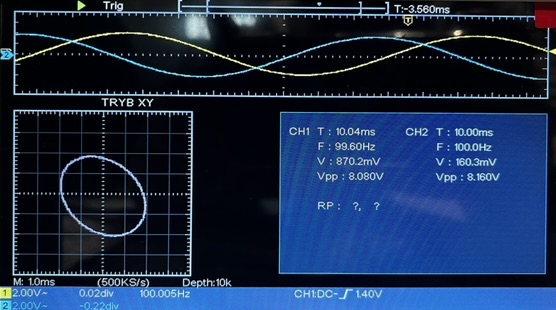
\includegraphics[width=3cm]{imagenes/liss_1_1.jpeg}
      & 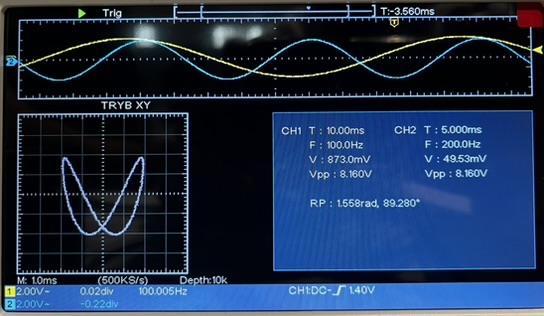
\includegraphics[width=3cm]{imagenes/liss_1_2.jpeg}
      & 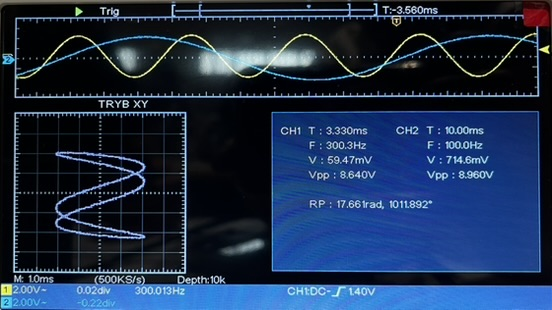
\includegraphics[width=3cm]{imagenes/liss_1_3.jpeg}
      & 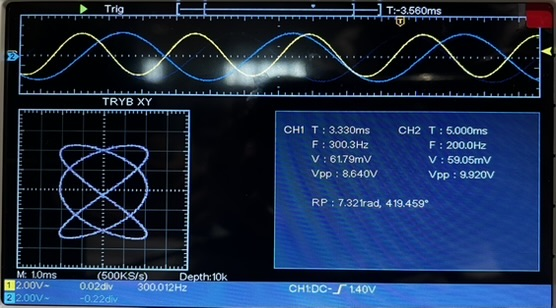
\includegraphics[width=3cm]{imagenes/liss_2_3.jpeg} \\
Frec.\ Canal 1 (Hz) & 100,0 & 100,0 & 100,0 & 200,0 \\
Frec.\ Canal 2 (Hz) & 100,0 & 200,0 & 300,3 & 300,3 \\
\bottomrule
\end{tabular}
\renewcommand{\arraystretch}{1.25}
\end{table}
\vspace{-0.3cm}

\noindent\textbf{3.\ Condiciones para que la figura de Lissajous sea una circunferencia.}

\medskip

Para que la composición de las dos señales~\eqref{eq:lissajous} forme una circunferencia deben cumplirse simultáneamente tres condiciones:

\begin{enumerate}
\item \textbf{Igual frecuencia:} $\nu_1 = \nu_2$ (equivalentemente $\omega_1 = \omega_2$), de modo que la relación de frecuencias sea $1{:}1$ y la trayectoria sea una cónica cerrada.

\item \textbf{Igual amplitud efectiva en pantalla:} $A = B$ tras ajustar las escalas de ambos canales para que la señal ocupe el mismo número de divisiones en los ejes $X$ e $Y$. Si $A \neq B$ la figura es una elipse.

\item \textbf{Desfase en cuadratura:} $\phi = \dfrac{\pi}{2} + k\pi$ con $k \in \mathbb{Z}$ (90° o 270°). Con $\phi = 0$ o $\phi = \pi$ la figura degenera en una recta; para valores intermedios resulta una elipse orientada.
\end{enumerate}

Con estas tres condiciones las ecuaciones paramétricas~\eqref{eq:lissajous} se reducen a:
\[
X = A\sin(\omega t), \qquad Y = A\cos(\omega t),
\]
de donde $X^2 + Y^2 = A^2$, ecuación de una circunferencia de radio $A$.

% ============================================================
\section{Ejemplo de cálculo}
% ============================================================

Para $f_{nom} = \SI{100}{\hertz}$, con escala horizontal \SI{2}{ms/div} y 5,00 divisiones entre crestas:
\begin{align*}
T_{rej} &= 5{,}00 \times \SI{2}{ms} = \SI{10{,}000}{ms} = \SI{0{,}01000}{s}, \\
\delta T_{rej} &= \frac{\SI{0{,}001}{ms}}{2} = \SI{5e-6}{s}, \\[4pt]
f_{rej} &= \frac{1}{\SI{0{,}01000}{s}} = \SI{100{,}00}{Hz}, \\
\delta f_{rej} &= \frac{\delta T_{rej}}{T_{rej}^{2}} = \frac{\SI{5e-6}{s}}{(\SI{0{,}01}{s})^{2}} = \SI{0{,}050}{Hz}.
\end{align*}

Para $V_{pp} = \SI{6{,}080}{V}$ con escala \SI{2}{V/div} y 3,04 divisiones:
\begin{align*}
V_p &= \frac{\SI{6{,}080}{V}}{2} = \SI{3{,}040}{V}, \qquad
\delta V_p = \frac{\SI{0{,}005}{V}}{2} = \SI{0{,}0025}{V}, \\[4pt]
V_{ef} &= \frac{\SI{6{,}080}{V}}{2\sqrt{2}} = \SI{2{,}150}{V}, \qquad
\delta V_{ef} = \frac{\SI{0{,}005}{V}}{2\sqrt{2}} = \SI{0{,}0018}{V}.
\end{align*}

Compatibilidad entre la medida automática y la de rejilla a \SI{50}{Hz}:
\[
C_{\text{auto},\text{rej}} = \frac{|49{,}969 - 50{,}00|}{\sqrt{0{,}013^2 + 0{,}001^2}} = \frac{0{,}031}{0{,}013} \approx 2{,}4,
\]
lo que muestra incompatibilidad ($C > 1$) si se usa la última cifra del display como incertidumbre de la medida automática.

\end{document}
